% !TeX spellcheck = en_US
% Created 2021-01-10 Sun 23:39
% Intended LaTeX compiler: pdflatex
\documentclass[11pt]{article}
\usepackage[utf8]{inputenc}
\usepackage[T1]{fontenc}
\usepackage{graphicx}
\usepackage{grffile}
\usepackage{longtable}
\usepackage{wrapfig}
\usepackage{rotating}
\usepackage[normalem]{ulem}
\usepackage{amsmath}
\usepackage{textcomp}
\usepackage{amssymb}
\usepackage{capt-of}
\usepackage{hyperref}
\usepackage{fancyhdr}
\usepackage{lastpage}

%Tot això hauria d'anar en un pkg, però no sé com és fa
\newcommand*{\assignatura}[1]{\gdef\1assignatura{#1}}
\newcommand*{\grup}[1]{\gdef\3grup{#1}}
\newcommand*{\professorat}[1]{\gdef\4professorat{#1}}
\renewcommand{\title}[1]{\gdef\5title{#1}}
\renewcommand{\author}[1]{\gdef\6author{#1}}
\renewcommand{\date}[1]{\gdef\7date{#1}}
\renewcommand{\baselinestretch}{1.5}
\renewcommand{\maketitle}{ %fa el maketitle de nou
	\begin{titlepage}
		\raggedright{UNIVERSITAT DE LLEIDA \\
			EPS \\
			Computer Engineering Degree, 4th\\
			\1assignatura, Computer Science\\}
		\vspace{5cm}
		\centering
		\huge{\5title \\}
		\vspace{3cm}
		\large{\6author} \\
		\normalsize{\3grup}
		\vfill
		Professors: \4professorat \\
		Date: \7date
\end{titlepage}}
%Emplenar a partir d'aquí per a fer el títol : no se com es fa el package
%S'han de renombrar totes, inclús date, si un camp es deixa en blanc no apareix

\title{Activity 6: REST WS}
\author{Joaquim Picó Mora, Ian Palacín Aliana, Sergi Simón Balcells}
\date{11th of January of 2021}
\assignatura{Distributed Computing}
\professorat{Eloi Gabaldon, Jordi Gervas, Josep Lluís Lèrida}
\grup{Computer Science}

\pagestyle{fancy}
\fancyhf{}
\lhead{Activity 6: REST WS}
\rhead{Page \thepage \hspace{1pt} of \pageref{LastPage}}


\begin{document}
	\maketitle
\thispagestyle{empty}
\newpage
\pagenumbering{roman}
\tableofcontents
\newpage
\pagenumbering{arabic}


\section{Introduction}
\label{sec:orgde35f88}
In this document is it specified all the endpoints and which responses
do they return, as well as a defense of which technologies we have used.
\\
\\
Additionally, it can be found a table containing the REST API developed,
as well as a class diagram of the database model used by the API.
\\
\\
The integration can be found at \href{https://github.com/sergisi/java-rmi/tree/integration}{RMI Project}, at
the branch \texttt{integration}. On the other hand, the Web Service can be found at
\href{https://github.com/quimpm/ws-distcomp}{WS Project}.

\section{UML}
\label{sec:org11252ab}
\begin{center}
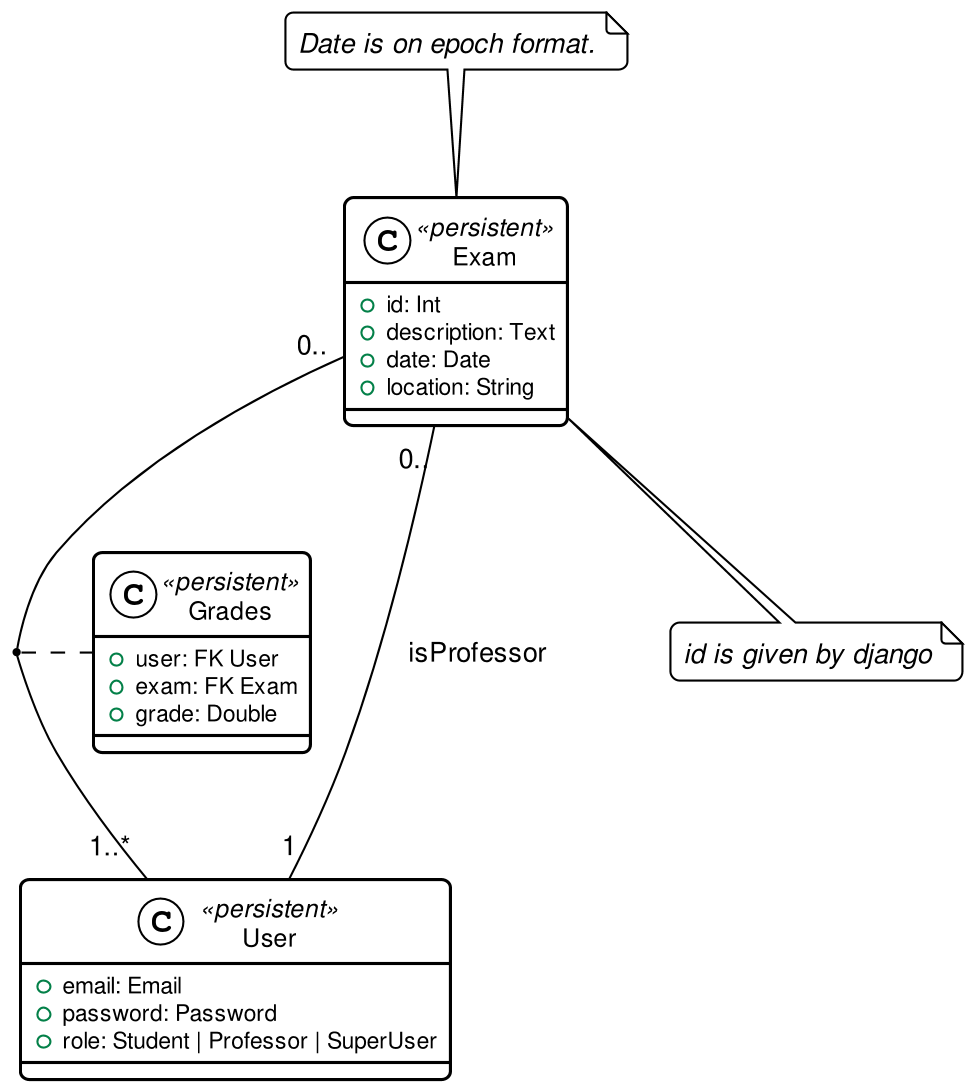
\includegraphics[width=.9\linewidth]{img/message_passing.png}
\end{center}

\subsection{Exam}
\label{sec:orgbcc73c2}
Exam is the class that holds all the Exam information. It stores the
a description, a date and a location of an exam.

\subsection{User}
\label{sec:orga01a2e5}
User is the class that stores the information of a user that is making
use of our system. It's the default implementation of the Django User
class.

\subsection{Grades}
\label{sec:org1e51923}
This class it's the one that stores grades of exams made by users. It holds two
foreign keys to the exam that belongs the grade, as well as the student.
\newpage
\section{Endpoint Table}
\begin{table}[h!]
\caption{Methods table (Part 1).}
\centering
\begin{tabular}{lp{4cm}p{5.5cm}l}
\hline
Method & URL & What & Status code\\
\hline
get & exam/ & List d'exams & 200\\
get & exam/\{exam\}/ & Detall de Exam (tot) & 200, 404\\
get & exam/search?description =\{text\}/ & Buscar descripció parcial. & 200\\
post & exam/ & Crea exam. pk no s'ha de donar. & 201, 403, 401\\
put & exam/\{exam\}/ & Modificar camps d'Exam (tots) & 200, 403, 401\\
patch & exam/\{exam\}/ & Partial update. & 200, 403, 401\\
delete & exam/\{exam\}/ & Deletes if professor and no grades & 204, 403, 401\\
\hline
post & grades/ & Penjar nota d'un examen. & 201, 403, 401\\
get & grades/\{user\}/user/ & List totes les notes d'un estudiant. & 200\\
get & grades/ & List all grades. & 200\\
get & grades/\{grade-id\} & Detail a grade. & 200, 404\\
put & grades/\{grade-id\} & Updates a grade. & 200, 403, 401\\
patch & grades/\{grade-id\} & Partially updates a grade. & 200, 403, 401\\
delete & grades/\{grade-id\} & Deletes a grade. & 204, 403, 401\\
\hline
\end{tabular}
\end{table}
\begin{table}
	\caption{Methods table (Part 2).}
\begin{tabular}{lp{4cm}p{5.5cm}l}
	\hline
	Method & URL & What & Status code\\
	\hline
post & auth/login/ & Logins & 201, 403, 401\\
get & auth/logout/ & Logouts & 200\\
post & auth/logout/ & Logout & 201, 403, 401\\
post & auth/password/change/ & Password change. & 201, 403, 401\\
post & auth/password/reset/ & Password reset by email confirmation. Needs Email configuration & 201, 403, 401\\
post & auth/password/reset /confirm/ & Password Confirmation & 201, 403, 401\\
post & auth/registration/ & Register a new user. & 201, 403, 401\\
post & auth/registration /verify-email & Verifies email. Needs Email configuration & 201, 403, 401\\
get & auth/user/ & Reads User. Needs authentication & 200\\
put & auth/user/ & Updates User & 200, 403, 401\\
patch & auth/user/ & Partial update. & 200, 403, 401\\
\hline
get & user/\{user\}/ & Gets user with pk. & 200, 404\\
\hline
\end{tabular}
\end{table}


\newpage
\section{Screenshots}
\label{sec:org3f54c26}
The screenshots are for the most important cases, there are endpoints
that has been omitted, like user password change.

Note that due to a bug in the docs viewer, as deleting an object only
returns a status code without any data, it does not correctly show that
the status code is 204. Instead, only shows ``undefined'', even though it
is properly deleted from the database.

\subsection{Authentication}
\label{sec:org20c7d93}
\begin{figure}[htbp]
\centering
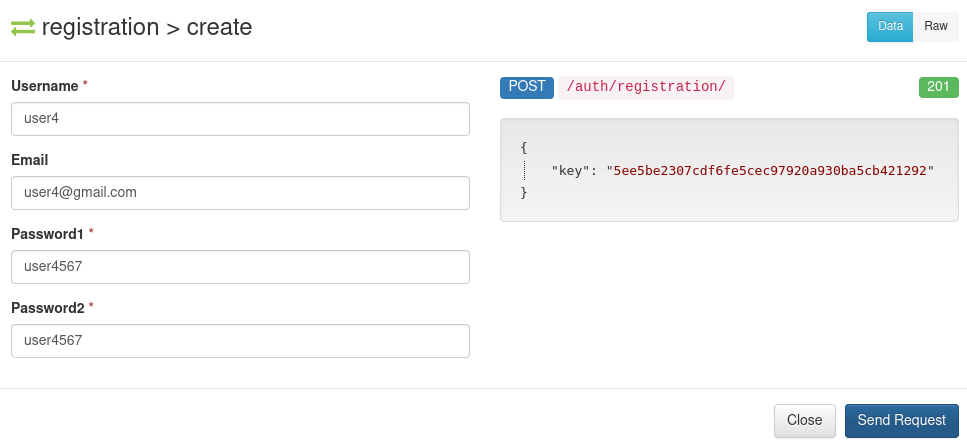
\includegraphics[width=.9\linewidth]{img/registration.png}
\caption{Register}
\end{figure}
\begin{figure}[htbp]
\centering
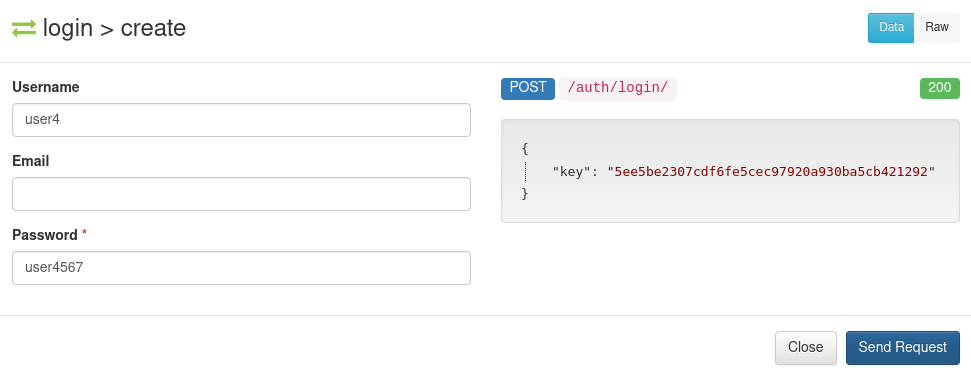
\includegraphics[width=.9\linewidth]{img/login.png}
\caption{Login}
\end{figure}

\newpage
\subsection{Exam}
\begin{figure}[h!]
\centering
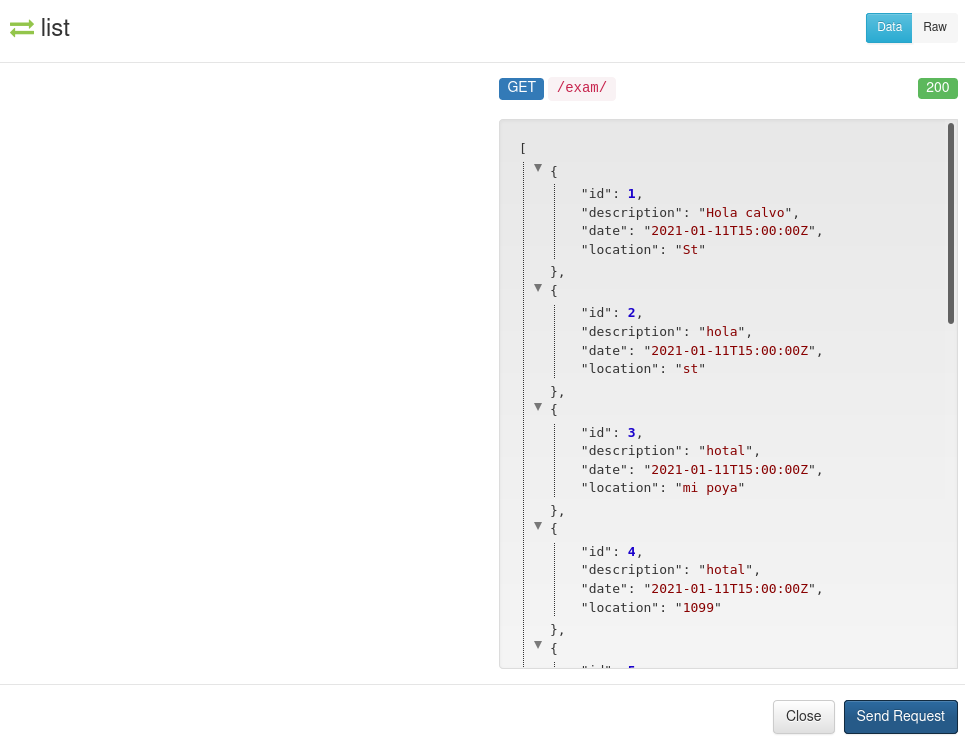
\includegraphics[width=.9\linewidth]{img/list_exams.png}
\caption{List exams}
\end{figure}
\begin{figure}[htbp]
\centering
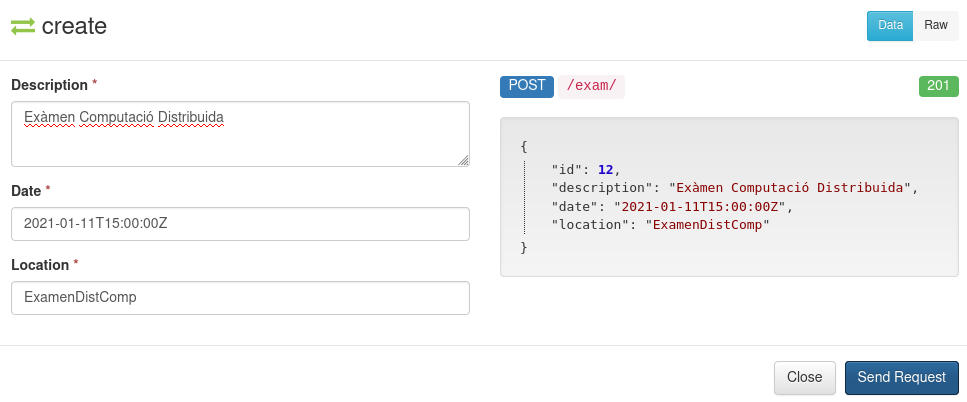
\includegraphics[width=.9\linewidth]{img/create_exam.png}
\caption{Create exam}
\end{figure}
\begin{figure}[htbp]
\centering
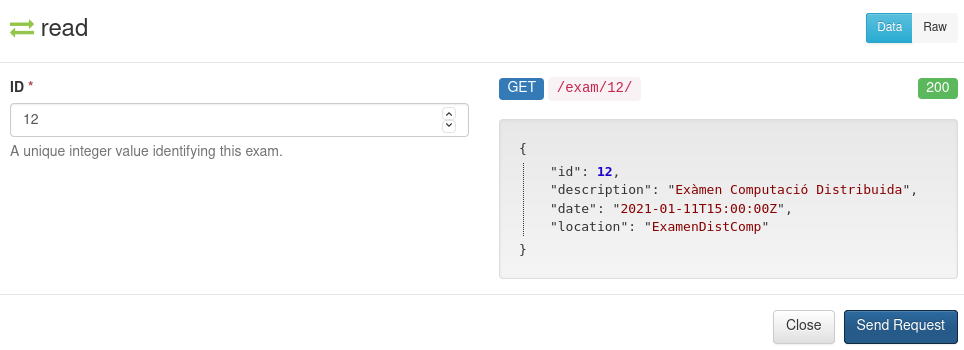
\includegraphics[width=.9\linewidth]{img/read_exam.png}
\caption{Read exam}
\end{figure}
\begin{figure}[htbp]
\centering
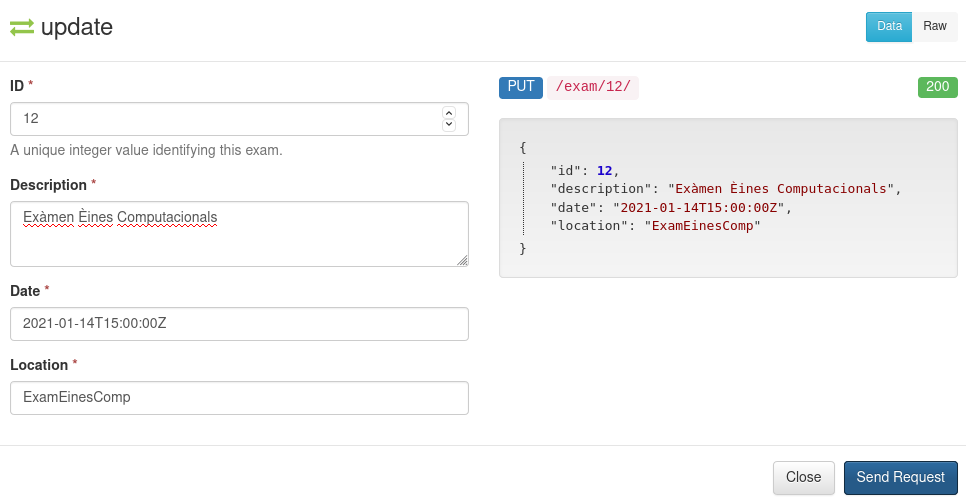
\includegraphics[width=.9\linewidth]{img/update_exam.png}
\caption{Update exam}
\end{figure}
\begin{figure}[htbp]
\centering
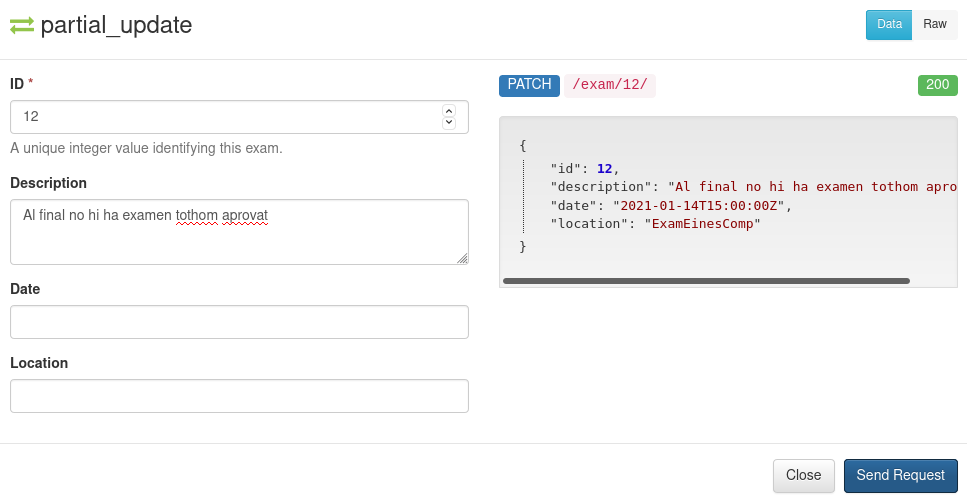
\includegraphics[width=.9\linewidth]{img/partial_update_exam.png}
\caption{Patch exam}
\end{figure}
\begin{figure}[htbp]
\centering
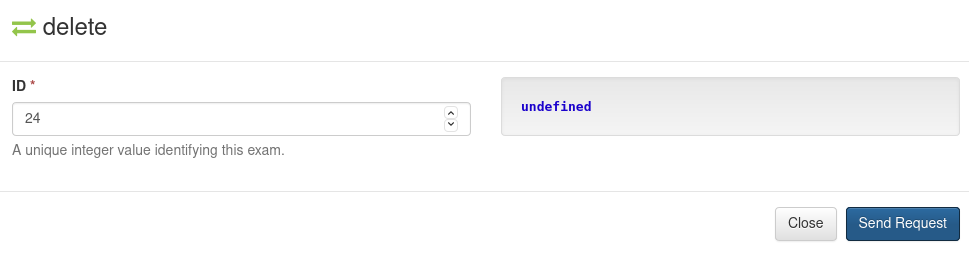
\includegraphics[width=.9\linewidth]{img/delete_exam.png}
\caption{Delete exam}
\end{figure}
\begin{figure}[htbp]
\centering
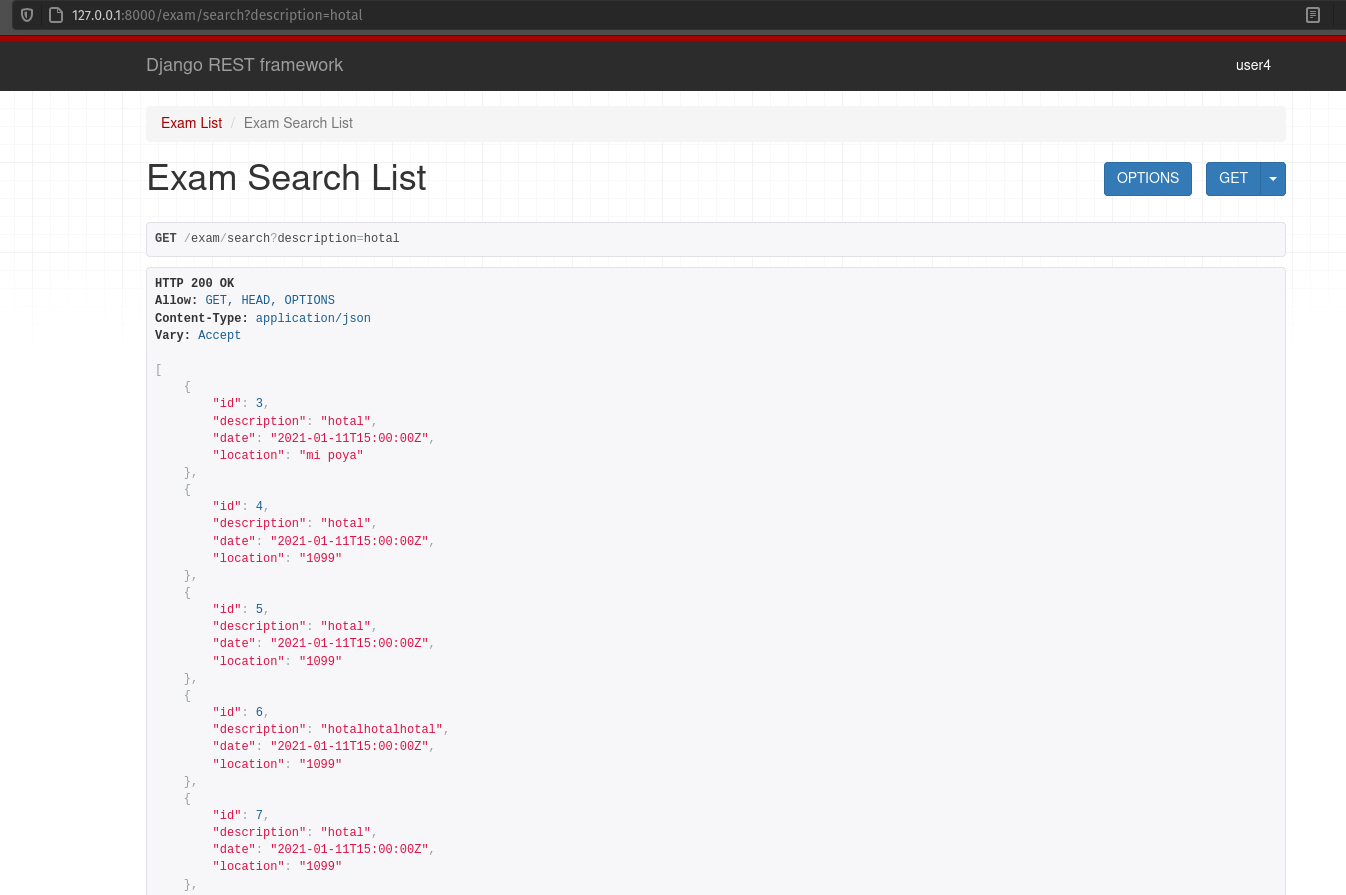
\includegraphics[width=.9\linewidth]{img/search1.png}
\caption{Search exam}
\end{figure}

\newpage
\subsection{Grades}
\label{sec:org0bbbe02}
\begin{figure}[h!]
\centering
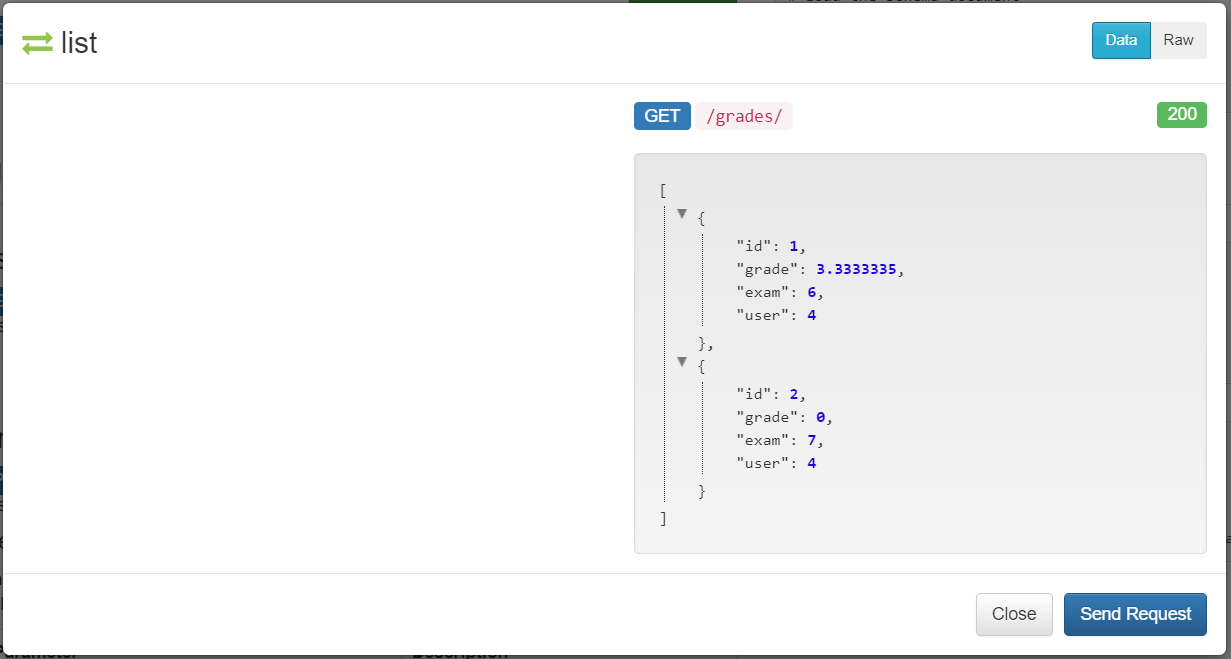
\includegraphics[width=.9\linewidth]{img/list_grades.png}
\caption{List grades}
\end{figure}
\begin{figure}[htbp]
\centering
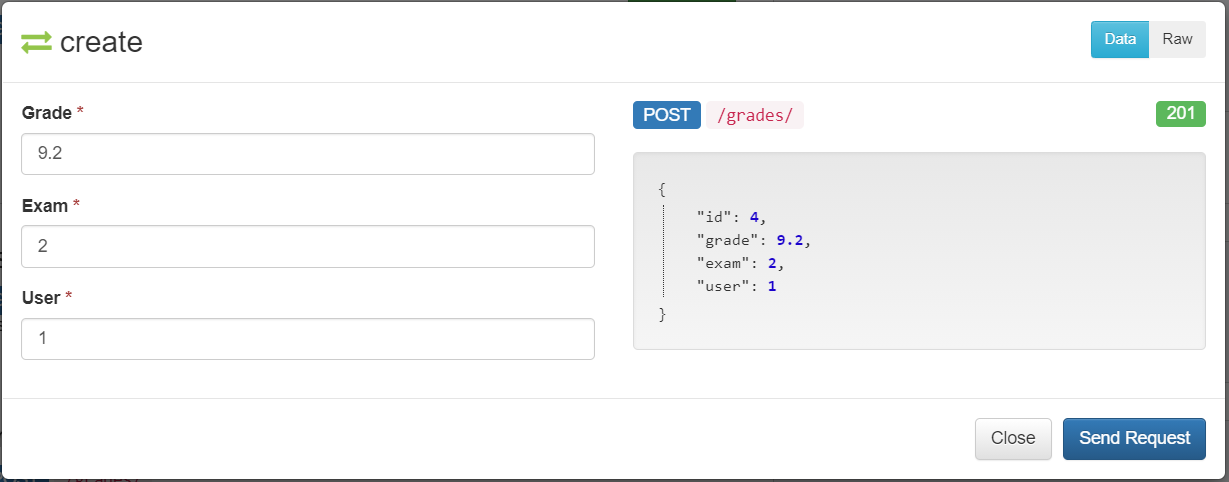
\includegraphics[width=.9\linewidth]{img/create_grades.png}
\caption{Create grade}
\end{figure}
\begin{figure}[htbp]
\centering
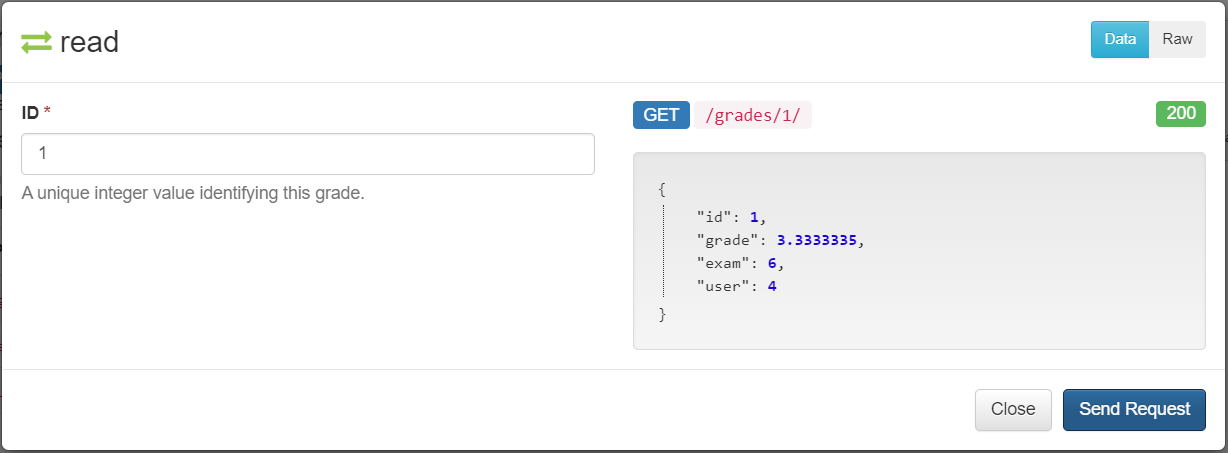
\includegraphics[width=.9\linewidth]{img/get_grades_by_id.png}
\caption{Read grade}
\end{figure}
\begin{figure}[htbp]
\centering
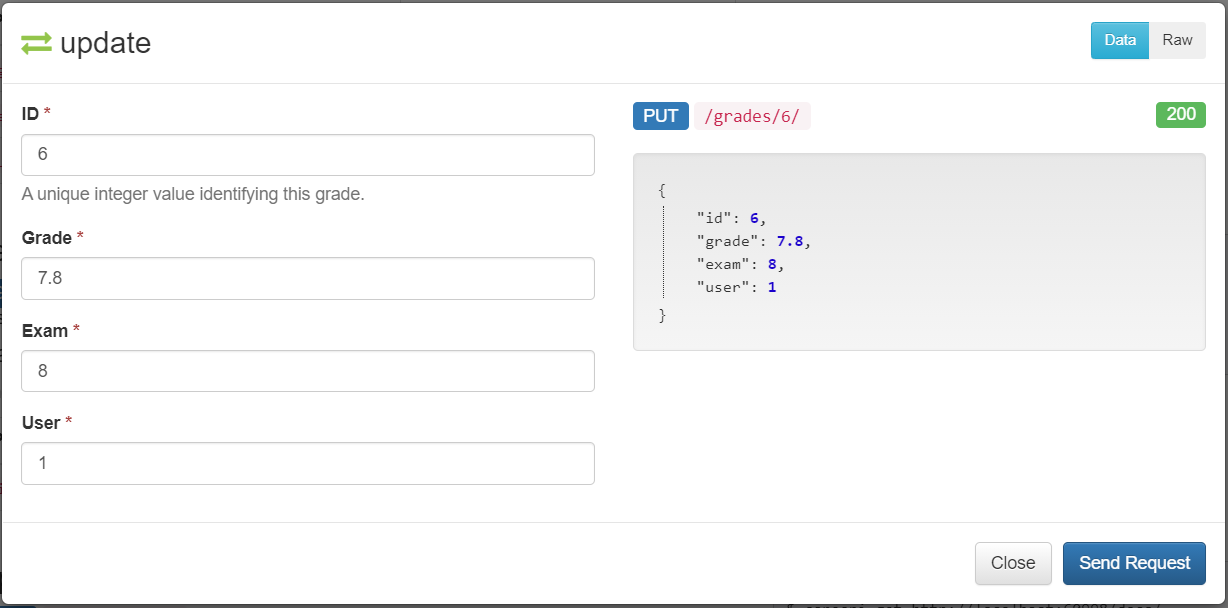
\includegraphics[width=.9\linewidth]{img/update_grade.png}
\caption{Update grade}
\end{figure}
\begin{figure}[htbp]
\centering
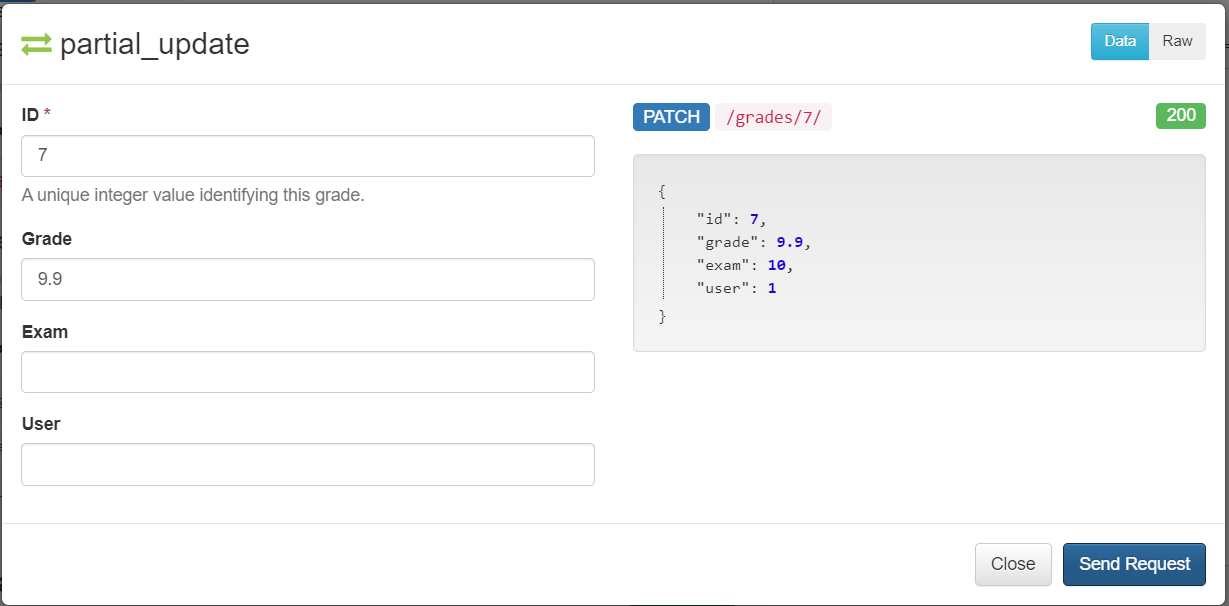
\includegraphics[width=.9\linewidth]{img/patch_grade.png}
\caption{Patch grade}
\end{figure}
\begin{figure}[htbp]
\centering
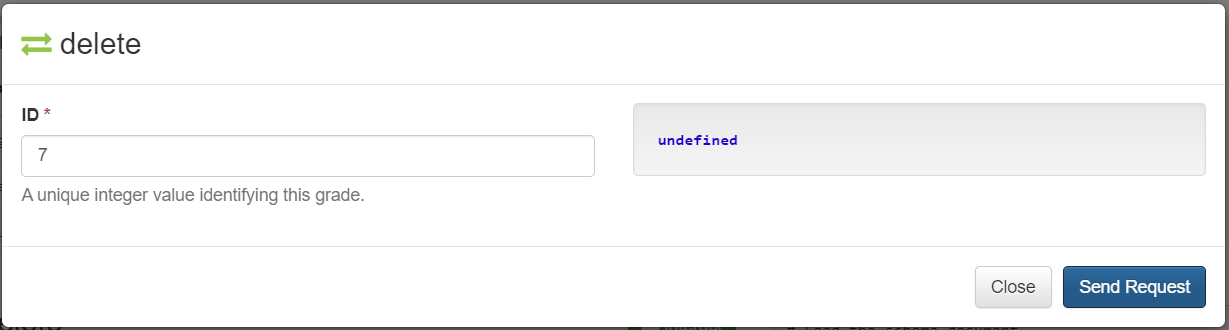
\includegraphics[width=.9\linewidth]{img/delete_grade.png}
\caption{Delete grade}
\end{figure}
\begin{figure}[htbp]
\centering
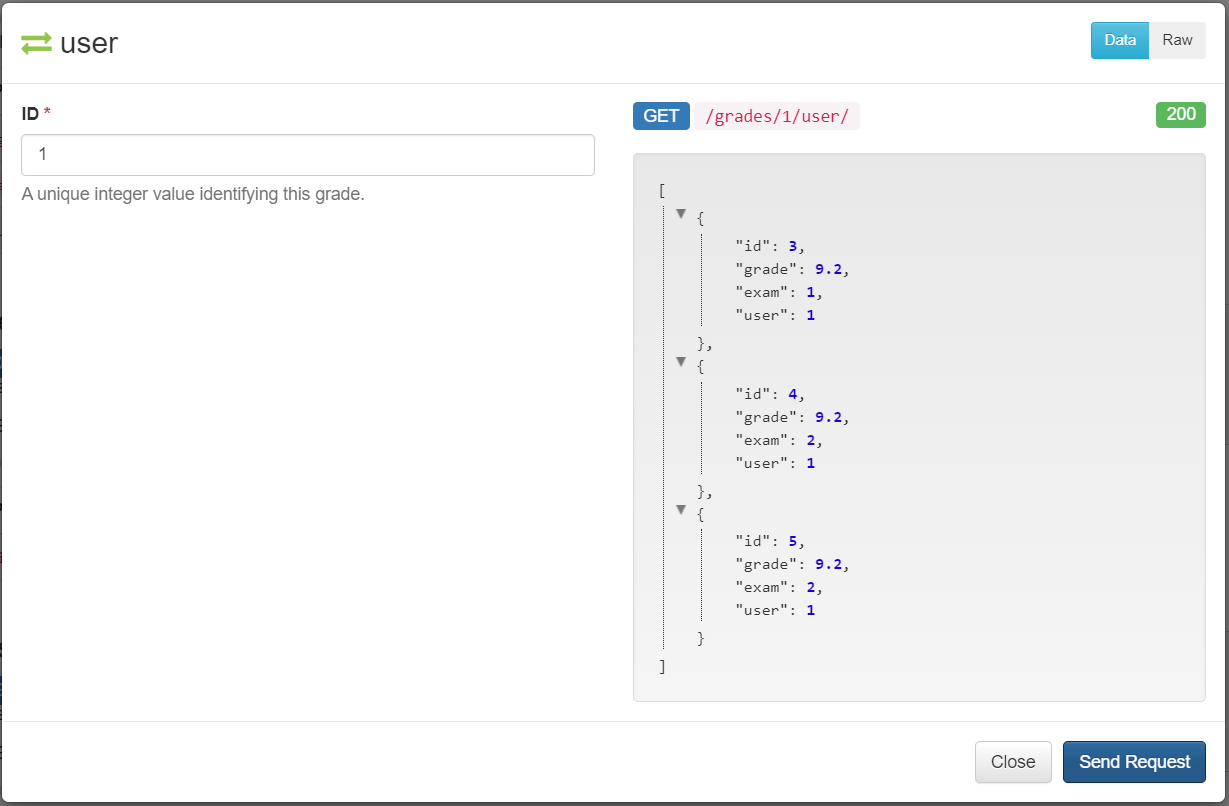
\includegraphics[width=.9\linewidth]{img/get_user_grade.png}
\caption{Search user grades}
\end{figure}
\begin{figure}[htbp]
\centering
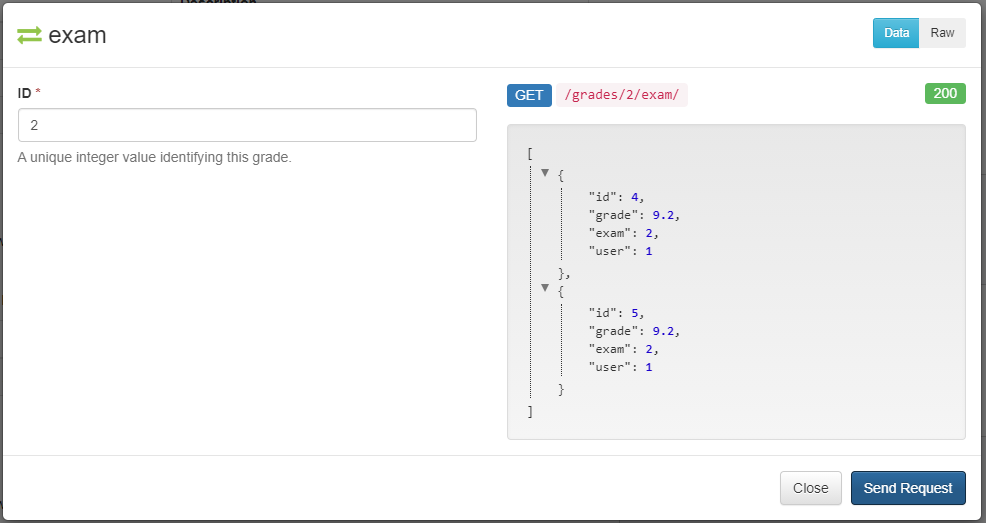
\includegraphics[width=.9\linewidth]{img/get_exam_grade.png}
\caption{Search exam grades}
\end{figure}

\newpage
\section{How To}
\label{sec:orgc1d500a}
\subsection{Getting Started}
\label{sec:orga657ce3}
These instructions will get you a copy of the project up and running on
your local machine for development and testing purposes. See deployment
for notes on how to deploy the project on a live system.

\subsubsection{Prerequisites}
\label{sec:org56cc4f8}
You will need to have installed docker and docker-compose. To know if
this is working properly use \texttt{docker run hello-world} and
\texttt{docker-compose -{}-version}. To get them installed properly at your OS,
refer to the official pages of docker and use:

\begin{verbatim}
  python3 -m pip install docker-compose
\end{verbatim}

\subsubsection{Installing}
Copy \texttt{example.env} to file named \texttt{.env}. Then change the variable
\texttt{DJANGO\_SECRET\_KEY=[key]} to a value generated. For example, using
\href{https://miniwebtool.com/django-secret-key-generator/}{this site}.

So the contents of \texttt{.env} should be:

\begin{verbatim}
  #Django configuration

  OPEN_PORT=8000
  DJANGO_PORT=8000

  DJANGO_SECRET_KEY=<your secret key goes here>
  DJANGO_DEBUG=1
  DJANGO_ALLOWED_HOSTS=localhost 127.0.0.1 [::1] 0.0.0.0

  POSTGRES_USER=postgres
  POSTGRES_PASSWORD=postgres
  POSTGRES_HOST=db
  POSTGRES_PORT=5432
  POSTGRES_NAME=postgres

  DATABASE_URL="postgres://$POSTGRES_USER:
  $POSTGRES_PASSWORD@$POSTGRES_HOST:
  $POSTGRES_PORT/$POSTGRES_NAME"

  EMAIL_OPTION=none
  EMAIL_USE_TLS=True
  EMAIL_HOST='smtp.gmail.com'
  EMAIL_HOST_USER='mail@gmail.com'
  EMAIL_HOST_PASSWORD='password1234'
  EMAIL_PORT=587
\end{verbatim}

Then apply the changes to your database using:

\begin{verbatim}
  docker-compose up -d
  docker-compose exec web python3 manage.py makemigrations
  docker-compose exec web python3 manage.py migrate
  docker-compose down
\end{verbatim}

To create a super user, use:

\begin{verbatim}
  docker-compose up -d
  docker-compose exec web python3 manage.py createsuperuser
  docker-compose down
\end{verbatim}

Then use \texttt{docker-compose up -d} to get it running. Connect to
\texttt{localhost:8000/admin} to see the admin login page, or
\texttt{localhost:8000/docs} to see the docs.
\\
\\
To stop it, use \texttt{docker-compose down}

\subsection{Running the tests}
\label{sec:orga7a521a}
To execute all tests, use
\texttt{docker-compose exec web python3 manage.py test}

\section{Solution justification}
\label{sec:orgf644e87}
\subsection{Web Service}
\label{sec:org3a6a157}
\subsubsection{Technologies}
\label{sec:org3f4b312}

\begin{description}
\item[{Django}] We have chosen this technology because our familiarity with it
and its ease to work with data models and ORM.

\item[{Django rest framework}] This framework is a powerful and easy-to-use
tool for building web REST API's, it includes mechanisms for
serialization and authentication, which we found necessary.

\item[{SQLite}] it is the Django default database. A PostgreSQL  can be
configured as a replacement for scalability and deployment purposes.
It is already specified in the environment, but was left as SQLite
was sufficiently for the requirements.

\item[{Docker}] It facilitates the encapsulation and execution of the
project, as it is contained in a container.

\item[{Docker-compose}] Easier configuration for a docker.
\end{description}

\subsubsection{ViewSets and Generics}
\label{sec:org512aace}
Django is an opinionated framework. With this, it provides powerful
abstraction if you can manage to use them. Django REST Framework, based
on it, \emph{copies} some of their abstractions and provides them for a
RESTful API. For example, in Django we extend View classes and add them
some information about which HTML template to use and which database
model, and it will pass correctly the data.\\
\\
With the REST framework, we have a similar idea. We have the concept of
generics, that provides a unique endpoint to an action, as retrieving an
object from the database or listing a few of them. When they did this,
they saw that most of their implementations used the same parameters:
where to get the objects and how to serialize them. And for this reason
they build what is called \texttt{ViewSets}. They provide an abstraction
to build all the \texttt{CRUD} operations of a model in the database. In
conjunction with the permissions class, they can provide a quick and
robust way to deploy the API. Most of our endpoints are made with this
\texttt{ViewSets}, the only ones that don't use them are
Filtering Views as they were made with a custom \texttt{ListAPIViews}  and a custom \texttt{get\_queryset} function.\\
\\
A user detail is not provided by the \texttt{auth} API, but it was needed for the 
presentation, so we made a custom endpoint to read a specific User.

\subsubsection{Decisions}
\label{sec:org0ef4455}

\begin{description}
\item[{Authentication}] We developed a simple authentication in which users
once registered and logged are provided with a token. This  provides
a way of authentication against some endpoints in the WS, as POSTs and DELETEs. 
There are custom permissions to prevent forbidden actions, like a student deleting an 
exam, or modifying a grade. We used \texttt{dj-rest-auth}, which provides endpoints for
registration, authentication, password reset, retrieve and update
user details, etc.

We also used \texttt{django-all-auth}, which implements a powerful back-end to
registration. It also provides with a plug-and-play of social
authentication, (i.e.: login with your Google account), and email
verification. Although we initially made an Email back-end, we needed
to provide in the environment either a usable email or an email
provider. We made a special parameter, so they are not needed, as we
thought that this will cause some trouble when correcting the project
rather than being a feature.
\end{description}

\subsection{RMI modifications}
\label{sec:org848e0b6}
\begin{description}
\item[{HTTP}] We have made two adapter classes in order to encapsulate the
HTTP requests made to the web service by the client and the server. To
make the request we have used \texttt{OkHttp3}, as we were restricted to use a
library from before Java 8 because of RMI deprecation in Java 9, but we initially intended
to use HTTP of Java 11. We were unable
to mock and test the API calls because \texttt{OkHttp3} Request and Response
object does not implement equals, and are final.

\item[{Client flow changes}] Now the client has to be identified in order to
enter the exam session, so the first step is to ask for a correct user
and password. Once authenticated correctly the user is given 3
options:

\begin{description}
\item[{search <keywords> }] searches exams by its description and outputs
the information of the matched exams.
\item[{list}] lists and outputs all the exams and its information.
\item[{choose <id-exam>}] chose the desired exam in order to connect to
its session. Once an exam is chosen, the flow works as before.
\end{description}

\item[{Server flow changes}] As happens with the client, the professor has
to be identified in order to create an exam session, so the first step
is to ask for a correct user and password. Once authenticated
correctly it will be asked to introduce the following parametters in
order to create the exam:

\begin{description}
\item[{description}] The description of an exam.
\item[{date}] Date of an exam. It needs a specific date format, as

\texttt{YYYY-MM-DDThh:mm:ssZ}.

\item[{location}] The location of an exam (string). We decided that the
location will be the bind key of the remote object that references
the exact exam session. Once the last parameter is filled, the
exam will be created in the web service, as well as the session in
which the students can connect to perform the exam. When a
professor finishes an exam, all the grades are uploaded to the web
service.
\end{description}
\end{description}

\subsection{Hours dedicated}
\label{sec:org2cca440}
It is difficult to say, but we estimate an approximation of 90 hours. We
are a group of three students, and we worked in this project for 6 days,
5 hours each day.
\end{document}
